\documentclass[output=paper]{langsci/langscibook} 
\ChapterDOI{10.5281/zenodo.1300624}
\author{Victoria Monje\affiliation{Universitat Pompeu Fabra}\lastand
Angelica Carlet\affiliation{Universitat Internacional de Catalunya}}
\title{The second time around: The effect of formal instruction on VOT production upon return from study abroad}
\shorttitlerunninghead{The effect of formal instruction on VOT production upon return from   abroad}
 
 
\abstract{The present study aims at assessing~L2 phonological development,~while controlling for proficiency level, as a result of~a 2-month formal instruction (FI) period following a 3-month period spent abroad in a country where the learners’ target language was spoken. It examines voice onset time (VOT) production of English voiceless stops in initial stressed position by Catalan/Spanish EFL learners. It is intended as a follow-up of \citegen{Mora2008} study, which yielded no significant effects at the end of the stay abroad (SA) only. It is hypothesized that the FI period should allow students to focus on their phonology, away from the pressing demands of daily communication during SA. No explicit attention is paid to phonology in class. Speech samples were collected from 13 participants, through two tasks, upon their return from SA and immediately after a 2-month period of FI. No significant effect of the FI period preceded by a SA term on informants’ VOTs was found. Proficiency level seems to have played a role in VOT production. Speaking style, vowel height and place of articulation were found to significantly affect VOT production of voiceless stops, in line with previous findings. A baseline group of natives showed the same numerical tendency.~The lack of impact resulting from a FI period preceded by a SA term adds further support for the suggestion made by some authors (\citealt{DarcyEtAl2012,GordonDarcy2012,CalvoBenzies2014}) that explicit attention to phonology in FI should act as a potential factor to effectively improve L2 phonological development.
}

\maketitle

\begin{document}






\section{Introduction}


It is often assumed that \isi{L2} oral \isi{speech development} will improve as a result of stay abroad (SA), whereas less improvement will be noted as a consequence of \isi{formal instruction} (\isi{FI}). However, there is little evidence to support this claim, as studies assessing second language (\isi{L2}) \isi{phonological} \isi{acquisition} resulting from a SA are still scarce and results are conflicting. Importantly, \isi{phonological} development seems to be one of the most challenging aspects of \isi{L2} \isi{acquisition} for learners, a fact that is likely due to a lack of a consistent pedagogical methodology in teaching \citep{DarcyEtAl2012}. 



Hence, this empirical study aims at continuing to fill the existing research gap in \isi{L2} \isi{speech production}. The study has been carried out within the \isi{Study Abroad} and Language Acquisition (SALA) project (see \citealt{Pérez-Vidal2014}), where \isi{linguistic} and non-\isi{linguistic} progress as a function of SA are analysed, including \isi{L2} \isi{phonological} development. \isi{FI} has also been examined in combination with SA within the project. However, \isi{FI} periods preceded SA ones in the SALA studies. Our work seeks to provide a counterbalanced perspective by examining the impact of an \isi{FI} period following a SA.



In order to obtain as thorough an understanding of \isi{L2} \isi{phonological} development as possible, the interplay of three important connected aspects is explored in the literature review: (i) the teaching of \isi{pronunciation} in the classroom, (ii) the \isi{linguistic} outcomes obtained as a \isi{function of learning context}, and (iii) \isi{voice onset time} (\isi{VOT}), which is the phenomenon under investigation in the present study. 



\section{Literature review} 


Pronunciation is often neglected in the \ili{English} as a second language (ESL) classroom despite its importance and interconnection with the four \isi{linguistic} skills \citep{DarcyEtAl2012}. Moreover, according to \citet{CalvoBenzies2014,CalvoBenzies2016}, \ili{English} \isi{pronunciation} can be seen as one of the most difficult skills to acquire and develop for \ili{Spanish} learners of \ili{English}. First language (L1) interference, an incoherent relation between spelling and \isi{pronunciation} and other non-\isi{linguistic} factors such as motivation, age and amount of exposure have been identified as factors to which such difficulties can be ascribed (\citealt{DarcyEtAl2012,CalvoBenzies2014}). The reasons that make the teaching of \isi{pronunciation} complex are numerous: for instance, the lack of systematicity regarding content and lack of time devoted to it in the FL classroom (\citealt{DerwingFoote2011}), undertrained teachers (\citealt{Derwing2010,FooteEtAl2011}) and paucity of teaching materials. Pronunciation is often neglected in syllabuses, which leads teachers to believe that spending time on it is unnecessary. 



\citet{DarcyEtAl2012} and \citet{CalvoBenzies2014} emphasize the need for \isi{pronunciation} to be taught systematically at different levels of \isi{proficiency} (from beginners to the most advanced learners). Additionally, \citet{GordonDarcy2012} advocate for the usefulness of drawing explicit focus to form in \isi{pronunciation} instruction. The lack of success in the \isi{acquisition} of \isi{L2} \isi{pronunciation} might partly be related to the little amount of attention it receives in the \isi{L2} classroom.



Due to the general lack of success of \isi{FI} in \isi{L2} \isi{phonological} development, SA is often considered a more appealing alternative to foster this \isi{linguistic} skill. In fact, when SA and \isi{FI} are compared, SA is said to be more advantageous regarding the quantity and quality of input it offers the learner. This constant exposure grounds the assumption that SA is more likely to lead learners to enhanced \isi{L2} knowledge than \isi{FI}. However, this does not seem to be the case for \isi{L2} \isi{phonological} development. In fact, there are reported cases of adults who, in spite of displaying a high command of their \isi{L2} due to a long length of stay abroad, still retain a distinct foreign \isi{accent} revealing \isi{phonetic} traits of their L1 (\citealt{DaltonSeidlhofer1994,FlegeFrieda1997}).



  Other factors that account for the (lack of) success in \isi{L2} \isi{phonological} development are the characteristics of each \isi{learning context}. According to \citet{Pérez-Vidal2014}, SA is a naturalistic \isi{learning context} in which exposure to the \isi{target language} is constant, which can potentially provide massive amounts of input, output and interaction opportunities. The case of \isi{FI} seems to be the opposite, due to its poorer input and limited opportunities for production. Therefore, one should expect different \isi{linguistic} outcomes from SA and \isi{FI}. SA spurs the enhancement of certain skills which are normally difficult to teach in \isi{FI}. The latter, in turn, tends to focus on aspects such as metalinguistic awareness and grammar. Thus, from the point of view of skill \isi{acquisition} theory, the classroom is the optimal environment for declarative knowledge to become procedural, whereas SA is ideal to reach automatization \citep[214]{DeKeyser2007study}. 



  In turn, success in \isi{L2} \isi{speech production} is subject to inter-speaker variability due to the interplay of several factors (e.g. motivation and cognitive abilities) \citep{Mora2014}. Mora suggests that having high motivation to learn the \isi{L2} makes learners more likely to interact with natives and hence gain access to richer input. The impetus for engaging in \isi{L2} encounters must then come from the learners themselves. Therefore, in-country residence does not guarantee quality input or interaction \citep{Moyer2009}, just as context of learning per se does not grant enhanced \isi{L2} production. Learners must also process the comprehensible input they receive in order to benefit from it, a notion known as intake \citep{Archibald2005}. This leads us to doubt the apparent superiority of the input received in SA over that obtained in \isi{FI}. 



  The idea that input during a SA may be insufficient to reach success in \isi{L2} \isi{phonological} \isi{acquisition} might be linked to the fact that the processing demands learners have to face leave them with few resources to focus on form. As opposed to \isi{FI}, SA is a meaning-oriented context. Other limitations to the quantity and quality of input in SA contexts are the (frequent) use of L1, fossilization and lack of feedback \citep{Han2004}.



  Lastly, the learner’s initial \isi{proficiency} level before the SA period also seems to play a role as far as \isi{L2} \isi{speech development} is concerned. There is a fairly acceptable degree of agreement on the fact that the learners’ initial \isi{L2} level might influence the accrued gains (if any) during their experience abroad \citep{Collentine2009}. This phenomenon is known as \textit{threshold} \textit{level}. Learners at a lower level make greater progress during SA than their higher level counterparts \citep{BrechtEtAl1995}. 



  Hence, \isi{learning context} is important, but it might not suffice to account for \isi{L2} \isi{speech development}. Moreover, each \isi{learning context} must be accurately defined to avoid misconceptions about the \isi{linguistic} results they trigger. More specifically, given the SALA project’s contradictory findings on different \isi{linguistic} skills as a \isi{function of learning context}, \citet[29-30]{Pérez-Vidal2014} concludes that skill development is not linear in a SA context, just as it is not in a \isi{FI} context. For example, learners show substantial progress in oral skills after a SA period (\citealt{López-Serrano2010}); however, research on \isi{L2} \isi{phonological} development is scarce and has failed to show a clear superiority of SA over \isi{FI}, yielding conflicting results (\citealt{Díaz-Campos2004,Avello2010a,SanzEtAl2013}).



  A study within the SALA project which especially captured our interest was that of \citet{Mora2008}. He looked at the effects of a SA period preceded by a \isi{FI} period on \isi{L2} \isi{phonological} development and the subsequent retention effects measured 15 months upon return from the SA. As for the specific abilities on focus, \isi{L2} production was studied, with \isi{VOT} of \ili{English} \isi{voiceless} \isi{plosive} consonants used to measure it. In addition, he also dealt with phonemic contrasts to test for perception accuracy. He found slight non-significant positive effects of SA on \isi{VOT} duration in \isi{voiceless} stops by \ili{Catalan}/\ili{Spanish} speakers after a period of \isi{FI}. That is to say, the positive effects were found only after the \isi{FI} period. The SA period was reported to have had positive influence on the \isi{VOT} production of those informants. 



  ESL learners with a \ili{Romance} language as their L1 tend to produce intermediate \isi{VOT} values that arise from cross-language influence in \isi{VOT} studies (\citealt{Flege1987,FlegeEtAl1998,ReisNobre-Oliveira2007,YavaşWildermuth2006,Mora2008,SchwartzhauptEtAl2014,AlvesZimmer2015}). It could be the case that \isi{VOT} does not take priority for learners, due to its allophonic character (\citealt{AlvesZimmer2015}). The Speech Learning Model (SLM) has provided so far the soundest basis to account for these results. It attributes \isi{L2} \isi{phonological} errors mostly to incorrect perception, although other causes are not discarded. More specifically, \citet{Flege1995} claims that the L1 and \isi{L2} categories coexist in a common \isi{phonological} space, inevitably influencing each other, leading hence to a bidirectional \isi{interlanguage} interaction. In this sense, the further apart an \isi{L2} sound is perceived to be from an L1 sound in that \isi{phonological} space, the more likely it is to be discerned. In contrast, if the L1 and \isi{L2} sounds are close to each other, category assimilation is said to take place. However, if there are cues which differ from one language to the other, learners might be sensitive to them. This is explained through the notion of categorical perception, because “even if listeners perceive two speech sounds as belonging to the same category, they subconsciously perceive a difference, as stimuli that fit better into a given category are easier and faster to process” \citep[25]{Bach2012}. This would ultimately lead to merged categories or intermediate values between the L1 and the \isi{L2}. This is the case of \isi{VOT}, which has hence been selected as an appropriate measure to shed light on \isi{L2} \isi{speech production} in the present study. \isi{VOT} has most generally been defined as “the interval between the release of the stop and the onset of glottal vibration, that is, voicing” (\citealt{AbramsonLisker1964}: 389). Interestingly, there is an overlap between \ili{English} voiced stops and \ili{Spanish} \isi{voiceless} stops at the phonemic level \cite{Yavaş2007}, which might confuse \ili{Spanish} learners of \ili{English}. In contrast, \ili{English} \isi{voiceless} stops find no equivalent in the \ili{Spanish} system. This explains the difficulty \ili{Spanish} learners face when acquiring the long lag of \ili{English} \isi{voiceless} stops. They normally produce \ili{English} \isi{voiceless} stops without their characteristic aspiration. See \citet{Yavaş2007} for a more detailed comparison between \ili{English} and \ili{Spanish} plosives.



  Although there is no absolute value for each \isi{plosive}, some authors (\citealt{KentRead1992,ToribioEtAl2005}) indicate that the standard \isi{VOT} patterns in \ili{English} are 55ms for /p/, 70ms for /t/ and 80ms for /k/. Importantly, these values apply only to stressed syllables in word-initial position (\citealt{ReisNobre-Oliveira2007}), as stress is a factor of variation in \isi{VOT} production. Normally, stops in unstressed syllables display lower \isi{VOT} values than their stressed counterparts (\citealt{AbramsonLisker1967}). In contrast, this value is of 30ms for the \isi{VOT} of word initial /p~t~k/ in \ili{Romance} languages \cite{Yavaş2007,SchwartzhauptEtAl2014}. ESL learners with a \ili{Romance} language as their L1 tend to produce \ili{English} word-initial \isi{voiceless} stops with a duration longer than 30ms, but shorter than typical native values. 



  Lastly, three independent factors have been found to affect \isi{VOT} duration: speaking rate, place of articulation and height of the preceding \isi{vowel}. Speaking rate has been found to be the most influential factor in \isi{VOT} variation; the faster one speaks, the shorter one’s \isi{VOT} values are (\citealt{ReisNobre-Oliveira2007,Mora2008,Bach2012}). Hence, speaking style has an effect on \isi{pronunciation}, an idea which comes originally from \citet{Labov1972}. This can therefore pose challenges to \isi{VOT} studies, given the difficulty to account for the variety in the speaking rate of informants. As for place of articulation, \isi{VOT} has been reported to increase “as the place of articulation progresses farther back in the oral cavity” \citep[260]{YavaşWildermuth2006}, which explains that velar stop consonants have the longest average \isi{VOT} (\citealt{ChoLadefoged1999}). Lastly, the height of the \isi{vowel} preceding the target stop might affect its \isi{VOT} value, with longer \isi{VOT} values found in the context of higher vowels than lower vowels (\citealt{FlegeEtAl1998,YavaşWildermuth2006}).



\section{The study}


The present study aims to provide a complement to the SALA project. Whereas the SALA project examined the impact of an SA period following a \isi{FI} period, in the current study, we focus on the effects of a \isi{FI} period following a SA period on \isi{L2} \isi{oral production} by a group of undergraduate \ili{Catalan}/\ili{Spanish} bilinguals. It is intended as a follow-up study based on \citegen{Mora2008} SALA study, which measured the effects of a SA period preceded by a \isi{FI} period on \isi{L2} \isi{phonological} development\footnote{Data collection times in \citegen{Mora2008} research were those of the SALA project: upon students’ enrolment (T1), after two terms of \isi{formal instruction} (about 80 hours) (T2), after a SA term (T3) in an \ili{English}-speaking country (this included about 40 hours of \isi{FI}), and 15 months later, after a two-term period without instruction/exposure to \ili{English}.}. Importantly, \isi{VOT} constitutes the only phenomenon explored in our research, unlike in \citet{Mora2008}, who also looks at the perception of \isi{vowel} contrasts. For this reason, \isi{VOT} is more thoroughly analysed here.



With the purpose of offering a counterbalanced view of his results, Time 2 and Time 3 in the data collection of the SALA project have been reversed in our study, resulting in Time 2 (T2) and Time 1 (T1), respectively. T1 in our data collection corresponds to the beginning of the period of \isi{FI}, and also the end of the SA period. T1 data were collected immediately after participants’ return from their SA. Then, after 2 months of \isi{FI}, Time 2 (T2) data collection took place. The data collected allow us to test whether the VOTs produced at pre-test and post-test significantly differ as a result of the \isi{FI} experience, preceded by a SA term. The impact of \isi{FI} (with no \isi{explicit attention} to \isi{pronunciation}) is the independent variable and \isi{VOT} duration of \isi{voiceless} \isi{plosive} \ili{English} consonants is the dependent variable. Additional independent variables explored are (i) \isi{proficiency} level, (ii) speaking style, (iii) \isi{vowel} height and (iv) place of articulation. 



Taking into account the difficulties for \isi{EFL} learners with \ili{Spanish}/\ili{Catalan} as their L1 to produce the correspondent aspiration of \ili{English} \isi{voiceless} stops, this study seeks to answer the following research questions (RQ) and states the corresponding hypotheses (H): 



\begin{description}
\item[\textbf{RQ1}.] Does a 2-month \isi{FI} period immediately following a 3-month SA period have an effect on the \isi{VOT} production of \isi{voiceless} \isi{plosive} consonants by \ili{Spanish}/\ili{Catalan} \isi{EFL} participants?

\item[\textbf{H1}.] The 2-month \isi{FI} period preceded by a SA term will have a positive though not necessarily large impact on the duration of the \isi{VOT} production of \isi{voiceless} stops by the advanced \ili{Spanish}/\ili{Catalan} learners tested. More specifically, informants are expected to produce higher \isi{VOT} values at T2 than at T1 but still not reaching native values, in line with the literature. 
\end{description}


In addition, \isi{proficiency} level (measured at T2) is addressed, as well as factors influencing \isi{VOT} production such as task effect (i.e. speaking style), \isi{vowel} height and place of articulation. In order to shed light on these issues, the research sub-questions (SRQ) below and their corresponding hypotheses (HSRQ) have been identified:


\begin{description}
 \item[\textbf{SRQ1.1.}] Do results vary when \isi{proficiency} level as measured through vocabulary size at T2 is taken into account? 

\item[\textbf{HSRQ1.1.}] No significant differences in \isi{VOT} values are expected as a function of \isi{proficiency} level as tested both after the SA and the \isi{FI} periods, in line with \citet{AlvesZimmer2015}. Any differences found triggered by this variable are expected to result in larger improvement by low level learners than by more advanced ones, following \citegen{Collentine2009} notion of \textit{threshold} \textit{level}.

\item[\textbf{SRQ1.2.}] Are there differences in the \isi{VOT} values as a \isi{function of task type} (i.e. speaking style) as measured through words produced in two different tasks (text reading-aloud task vs. carrier sentence task)?\footnote{\textsuperscript{} A series of sentences containing target words to be elicited.}

\item[\textbf{HSRQ1.2.}] The \isi{VOT} values obtained from the read-aloud text are expected to be shorter than those gathered from the carrier phrase task, as \isi{VOT} values tend to decrease in continuous speech in contrast with words uttered in isolation\footnote{Words elicited in the carrier-phrase task cannot be considered to be in complete isolation. See section 4.2 for a more detailed explanation of the purpose of each task.} (\citealt{Labov1972,Mora2008,Bach2012}).

\item[\textbf{SRQ1.3.}] Are there differences in the \isi{VOT} values as a function of the height of the \isi{vowel} following the target \isi{voiceless} \isi{plosive} consonant?

\item[\textbf{HSRQ1.3.}] Longer \isi{VOT} values are expected in the context of high vowels as opposed to low ones, according to Flege et al. (1998).

\item[\textbf{SRQ1.4.}] Does place of articulation have an effect on \isi{VOT} duration?

\item[\textbf{HSRQ1.4.}] Higher \isi{VOT} values will be obtained for /k/ than for the other stops as a function of place of articulation. In turn, the shortest \isi{VOT} values are expected to be obtained for /p/, according to \citet{YavaşWildermuth2006}.

\end{description}


\section{Method}


\subsection{Participants} %4.1



Thirteen undergraduate students from a university in Barcelona were recruited for the present study (11 females and 2 males\footnote{\textsuperscript{} The fact that the vast majority of participants are females is due to the high number of females taking the degree informants were recruited from. As a consequence, it was not possible to have a balanced amount of males and females. This also prevented us from studying possible gender effects.}, mean age = 19.1, \textit{SD} = 0.49).



As for language dominance, all participants are \ili{Spanish}/\ili{Catalan} bilinguals. However, not all of them report feeling equally dominant in both languages (see \figref{fig:monje:1}). More than a half feel \ili{Catalan}-dominant, according to the answers they provided to the questionnaire they were administered.



\definecolor{rosso}{RGB}{220,57,18}
\definecolor{giallo}{RGB}{255,153,0}
\definecolor{blu}{RGB}{102,140,217}

\begin{figure}
% https://tex.stackexchange.com/questions/135393/how-to-draw-bar-pie-chart
% 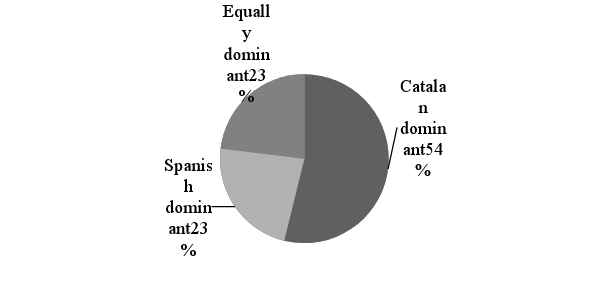
\includegraphics[width=\textwidth]{figures/monje-img1.png}
\begin{tikzpicture}
[
    pie chart,
    slice type={equal}{lsMidBlue},
    slice type={spanish}{lsDarkBlue},
    slice type={catalan}{lsLightBlue}, 
    pie values/.style={font={\small}},
    scale=2
]

    \pie{}{23/equal,23/spanish,54/catalan} 

    \legend[shift={(2cm,7mm)}]{{\ili{Spanish} dominant}/spanish, {equally dominant}/equal,  {\ili{Catalan} dominant}/catalan}

\end{tikzpicture}

\caption{\label{fig:monje:1} Self-reported language dominance}
\end{figure}
  






Participants belong to the institution’s intact groups, which are organized on the basis of an online entrance test pitched at a B2-C1 level. However, in order to check the real homogeneity of the group, an X/Y\_lex vocabulary size test was administered (see \citealt{Meara2005} and \citealt{MearaMiralpeix2006} for thorough descriptions of this test), showing that our participants differed in their lexical competence. Making claims as to the informants’ \isi{proficiency} level by looking only at their lexical knowledge would result in oversimplification, since other areas such as \isi{grammatical} and \isi{pragmatic} knowledge, for instance, would be neglected. However, for the purpose of this investigation, vocabulary size was judged to be an adequate proxy for general \isi{linguistic} \isi{proficiency} \citep{Milton2010}; considering that the main focus of the study is \isi{pronunciation}, and that it has been shown to have a relatively weak correlation with general language \isi{proficiency}, it was considered unnecessary to make participants undergo a time-consuming language \isi{proficiency} test. Following previous studies that use X/Y lex vocabulary test as a \isi{proficiency} measure (e.g. \citealt{Meara2005} and \citealt{MearaMiralpeix2006}), the test scores are divided into different ranges that correspond to the \isi{proficiency} levels set by the Common European Framework of Reference for Languages (CEFR). See \tabref{tab:monje:1} for correspondences.


\begin{table}
\caption{\label{tab:monje:1} Vocabulary size following common European Framework for Reference: X\_Lex Score equivalences}
\begin{tabularx}{.8\textwidth}{XX}
\lsptoprule

{Vocabulary size} & CEFR level\\
\midrule
 <1500 &    A1\\
 1500-2500   & A2\\
 2750-3250   & B1\\
 3250-3750   & B2\\
 3750-4500   & C1\\
 4500-5000   & C2\\
\lspbottomrule
\end{tabularx}
\end{table}


According to the vocabulary size test results, participants were placed into three different levels of CEFRL \isi{proficiency}, A, B and C (see \figref{fig:monje:2}). As it can be observed, 46\% of the participants have a C level, four of which fall in the C2 range. The score of the other two participants corresponds to the C1 level. Of the 39\% of learners who have a B level two learners fall in the B2 range and the other three at a B1 level. A learner scoring at an A1 level and another one at an A2 level constitute the 15\% scoring within the A level range.



  
\begin{figure}
%%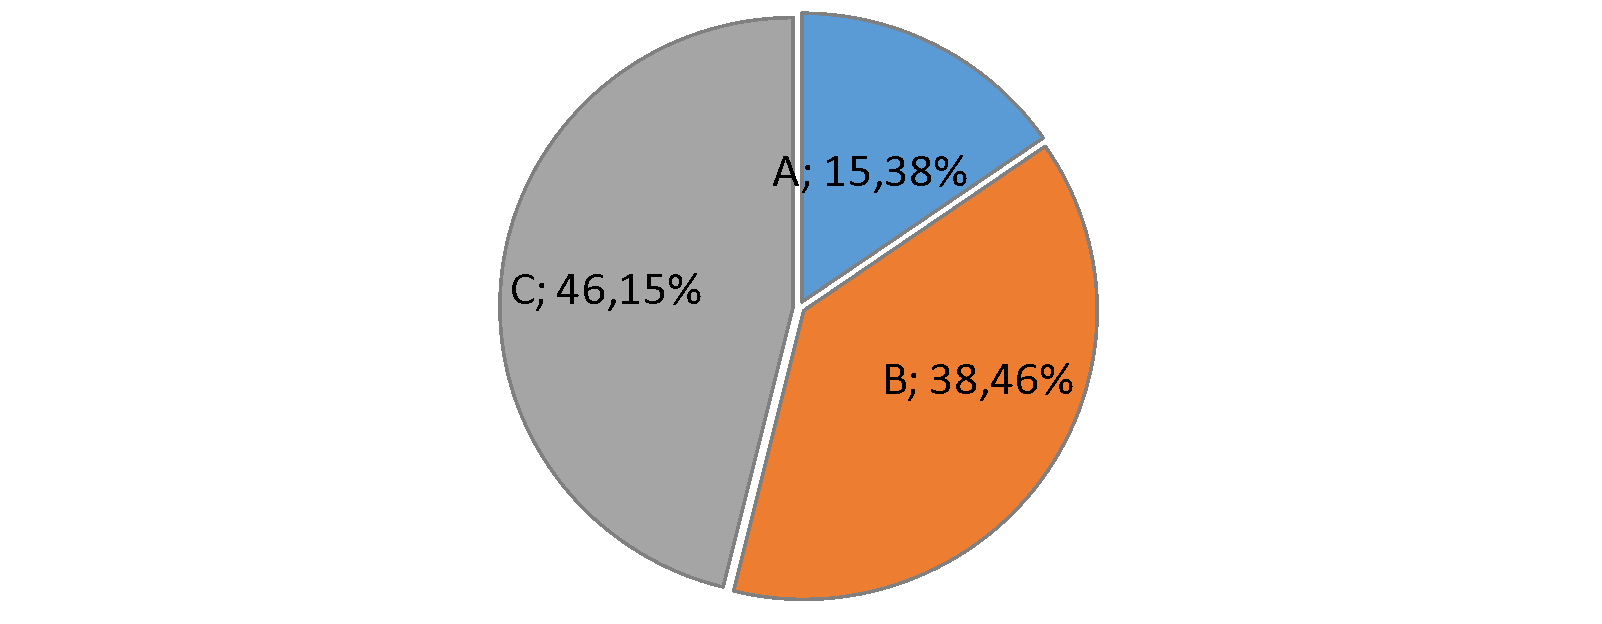
\includegraphics[width=\textwidth]{figures/monje-img2.png}
\begin{tikzpicture}
[
    pie chart,
    slice type={A}{lsMidBlue},
    slice type={B}{lsDarkBlue},
    slice type={C}{lsLightBlue}, 
    pie values/.style={font={\small}},
    scale=2
]

    \pie{}{15.38/A,38.46/B,46.15/C} 

%     \legend[shift={(2cm,7mm)}]{{X}/A, {Y}/B,  {Z}/C}

\end{tikzpicture}
\caption{\label{fig:monje:2}. CEFR proficiency level according to vocabulary size} 
\end{figure}



   Three native speakers participated in the study as a baseline group (2 female, 1 male; mean age = 24.8, \textit{SD} = 0.58). They all share a similar \isi{linguistic} background, as they are \isi{linguistic} majors and have a high command of two foreign languages, namely \ili{Spanish} and French. Two participants are speakers of American \ili{English} and the third participant is a speaker of Hiberno-\ili{English}. For the purpose of this investigation, it is considered that \isi{VOT} values do not differ as a function of language variety among native speakers, as they produce native-like values (i.e. above 60ms) (\citealt{LowensteinNittrouer2008}). 



\subsection{Procedure, tasks and stimuli}



The factors found to influence \isi{VOT} production mentioned above are taken into account in the present study (i.e. speaking style, \isi{vowel} height and place of articulation). Speech samples were obtained for subsequent acoustic analysis. \isi{VOT} was the segmental measure under scrutiny. Only \isi{voiceless} stops in word-initial position and followed by a stressed \isi{vowel} were included in the \isi{VOT} analysis. Thirty-one word-initial \isi{voiceless} stops produced three times by each of the 16 subjects (13 learners and three natives) at two data collection times were measured.



Participants were recorded in high quality sound-proof booths with the Audacity software and a \textit{Rode} \textit{NT-1AX} microphone. They were instructed to complete two tasks:  a carrier sentence task (isolated target words embedded in a carrier sentence – i.e. \textit{I} \textit{say} \textit{X,} \textit{I} \textit{say} \textit{X} \textit{now,} \textit{I} \textit{say} \textit{X} \textit{twice}) and a read aloud task (target words embedded in a text to be read continuously). The carrier-sentence/ read-aloud tasks were conceived to test participants’ \isi{VOT} production of word-initial stops in stressed syllables. Participants were instructed to articulate the stimuli as clearly as possible in both tasks, but especially the target words present in the carrier-sentence task.



Thirty-one monosyllabic words starting with a \isi{voiceless} stop (/p, t, k/) were selected for the test. There were 29 distractors, resulting in a total of 60 words. Vowel height was taken into account, as it is an influencing factor in \isi{VOT} production (\citealt{YavaşWildermuth2006}). Of the 11 words starting with /p/, the stop was followed by a high \isi{vowel} in five of the items (\textit{peach,} \textit{pill,} \textit{pear,} \textit{pin,} \textit{pig}) and by a low \isi{vowel} in six of them (\textit{pub,} \textit{pan,} \textit{park,} \textit{pup,} \textit{part,} \textit{pun}). Of the ten words starting with /t/, the stop was followed by a high \isi{vowel} in five instances (\textit{tear,} \textit{tip,} \textit{two,} \textit{ten,} \textit{tent}) and by a low \isi{vowel} in five of them (\textit{tan,} \textit{tuck,} \textit{touch,} \textit{tart,} \textit{toss}). As for the ten words starting with /k/, the stop was followed by a high \isi{vowel} in five cases (\textit{key,} \textit{could,} \textit{kill,} \textit{kilt,} \textit{kit}) and by a low one in the remaining five (\textit{cod,} \textit{card,} \textit{cot,} \textit{cap,} \textit{cut}). See \tabref{tab:monje:2} for a complete stimuli list. Distractors are presented in \tabref{tab:monje:3}. The 60 items were randomized and displayed in a PowerPoint presentation for the carrier-sentence task.


\begin{table}
\caption{\label{tab:monje:2}. Stimuli list for carrier sentence task}


\begin{tabularx}{.66\textwidth}{X@{}l X@{}l X@{}l}
\lsptoprule

\multicolumn{2}{c}{ /p/} & \multicolumn{2}{c}{ /t/} & \multicolumn{2}{c}{ /k/}\\
 HV & LV & HV & LV & HV & LV\\
 \midrule 
 \textbf{peach} & \textbf{pub} & tear & \textbf{tan} & \textbf{key} & \textbf{cod}\\
 \textbf{pill} & pan & tip & tuck & \textbf{could} & \textbf{card}\\
 pear & \textbf{park} & \textbf{two} & touch & kill & cot\\
 pin & pup & \textbf{ten} & \textbf{tart} & kilt & cap\\
 pig & part & tent & toss & kit & cut\\
\multicolumn{1}{c}{} & pun & \multicolumn{4}{c}{}\\ 
\lspbottomrule
\end{tabularx}

\end{table}


\begin{table}
\caption{\label{tab:monje:3} Distractors for carrier sentence task}

\begin{tabularx}{\textwidth}{XXXXXX}
\lsptoprule 
 bark & group & Bart & dart & beach & Dutch\\
 duck & do & bun & ghee & grew & gap\\
 God & big & dent & bear & dear & ban\\
 Dan & den & got & doss & guilt & bin\\
 Bill & good & guard & gut & dip & \\
\lspbottomrule
\end{tabularx}
\end{table}


   The second task was a text designed to be read aloud naturally with the purpose of taking into account the effect of speaking style. In order to do so, 12 items starting with a \isi{voiceless} stop were selected (in bold in \tabref{tab:monje:2}), four of which begin with /p/ (\textit{pill,} \textit{peach,} \textit{pub,} \textit{park}), four with /t/ (\textit{two,} \textit{ten,} \textit{tan,} \textit{tart}) and four with /k/ (\textit{keys,} \textit{could,} \textit{cod,} \textit{card}). In 6 items, the stop was immediately followed by a high \isi{vowel} (\textit{key,} \textit{ten,} \textit{could,} \textit{pill,} \textit{two,} \textit{peach}) and in the other 6, the stop was immediately followed by a low \isi{vowel} (\textit{tan,} \textit{park,} \textit{pub,} \textit{cod,} \textit{tart,} \textit{card}). The text was printed and physically handed to the participants for them to read aloud. 



The tasks were administered in two different orders with the purpose of counterbalancing task effects. In Order 1 the carrier sentence task was performed first, whereas in Order 2, participants started by reading the text. They were asked to read the text as naturally as possible. Additionally, at T1 the learners completed the Carlet-SALA questionnaire, a \isi{language background questionnaire} that resulted from the combination of the questionnaire used in \citet{Carlet2017} and the SALA questionnaire on SA conditions. They did so once they had performed the task. Lastly, they performed the vocabulary size test (\citealt{Meara2005,MearaMiralpeix2006}) at T2.



\section{Results and discussion}


\subsection{{Research question 1}}



Given the sample size, Wilcoxon signed-rank nonparametric tests for related samples were performed. As shown in \tabref{tab:monje:4} and \figref{fig:monje:3}, participants displayed slightly longer \isi{VOT} values at T2 than at T1. However, the 2-month \isi{FI} period immediately following a 3-month long SA period was found to have no statistically significant effect on the \isi{VOT} production of \isi{voiceless} \isi{plosive} consonants (\textit{z} = 0.384, \textit{N} = 13, \textit{p} = .3505, one-tailed).  



  Similar results were also obtained when analysing the two tasks separately. As can be seen in \tabref{tab:monje:4} and \figref{fig:monje:3}, participants displayed slightly longer \isi{VOT} values at T2 than at T1 for both tasks. A further Wilcoxon-test was run in order to reveal whether this difference reached statistical significance. Again, the 2-month \isi{FI} period immediately following a 3-month long SA term was found to have no statistically significant effect on the \isi{VOT} production of \isi{voiceless} \isi{plosive} consonants in either the text (\textit{z} = 0.314, \textit{N} = 13, \textit{p} = .3765, one-tailed) or the carrier sentence task (\textit{z} = 0.454, \textit{N} = 13, \textit{p} = .325, one-tailed). 


\begin{table}
\caption{\label{tab:monje:4} Mean VOT measurements (ms) at both testing times (T1, T2)}


\begin{tabularx}{\textwidth}{X rrrrSr}
\lsptoprule

 & \multicolumn{4}{c}{ \textbf{Non-native speakers}} & \multicolumn{2}{c}{ \textbf{Native \ili{English} speakers}}\\
  &  \textbf{T1 ms}  &  \textbf{(sd)} &    \textbf{T2 ms}  &   \textbf{(sd)} & \textbf{ms}  &  \textbf{(sd)}\\
  \midrule 
 {Both tasks} & 51.05& (20.39) & 51.54 &(18.13) & 65.47& (24.94)\\
 {Words}      & 54.93& (23.55) & 55.07 &(20.13) & 67.96& (29.87)\\
\lspbottomrule
\end{tabularx}
\end{table}

  
\begin{figure}
% 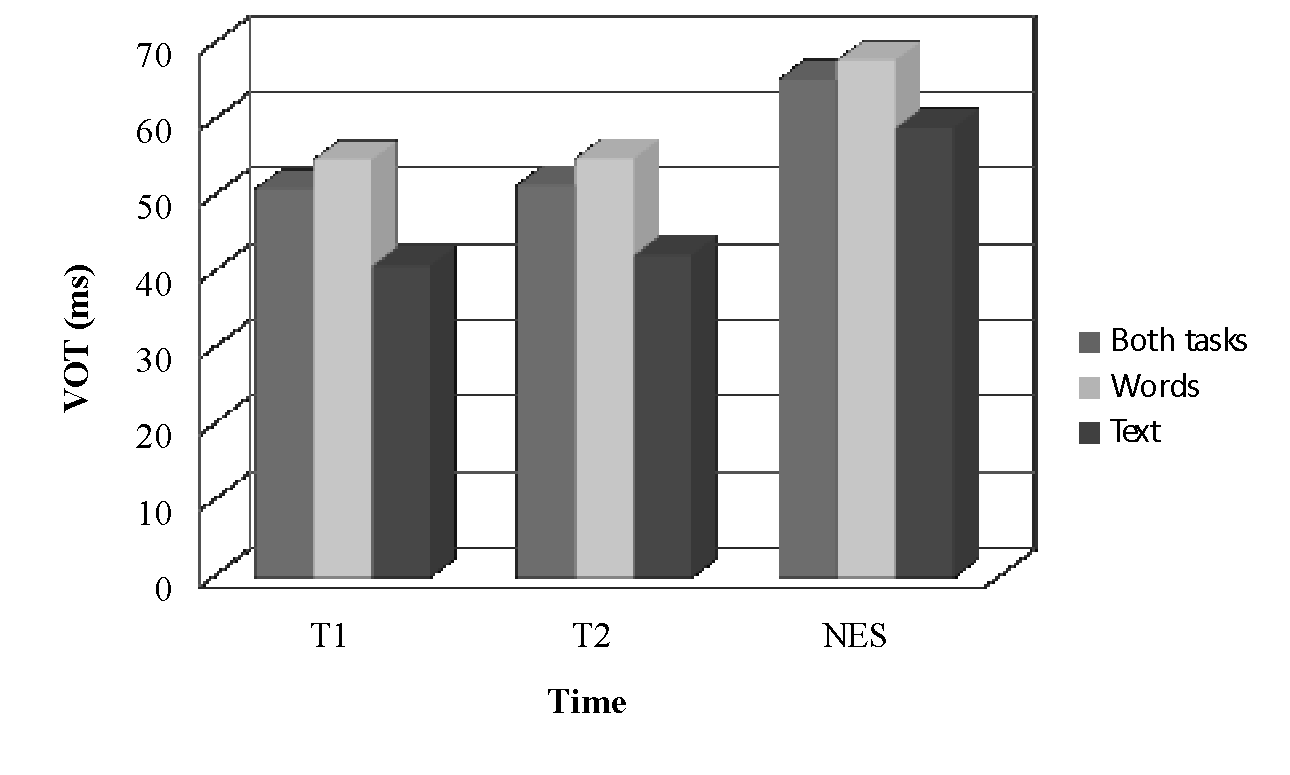
\includegraphics[width=\textwidth]{figures/monje-img3.png}
  \begin{tikzpicture}
    \begin{axis}[
	xlabel={Time},  
	ylabel={\isi{VOT} (ms)}, 
	axis lines*=left, 
        width  = .8\textwidth,
	height = .3\textheight,
    	nodes near coords, 
	xtick=data,
	x tick label style={},  
	ymin=0,
	ybar,
 	bar width=8mm,
	enlarge x limits=0.3,
	symbolic x coords={T1, T2, NES},
	legend style={at={(1,0.4)},anchor=west}
	]
	\addplot+[ybar,lsLightBlue!80!black,fill=lsLightBlue] plot coordinates {
	    (T1,51.05) (T2,51.54) (NES,65.47)
	}; 
	\addplot+[ybar,lsMidBlue!80!black,fill=lsMidBlue] plot coordinates {
	    (T1,54.93) (T2,55.07) (NES,67.96)
	}; 
	\addplot+[ybar,lsDarkBlue!80!black,fill=lsDarkBlue] plot coordinates {
	    (T1,40.99) (T2,42.40) (NES,59.06)
	}; 
	\legend{both tasks, words,text}
    \end{axis} 
  \end{tikzpicture}  
  
\caption{\label{fig:monje:3} Mean VOT measurements (ms) at both testing times (T1, T2)}
\end{figure}
 






These results may be interpreted as follows: The lack of explicit focus on \isi{L2} \isi{phonology} in the \isi{FI} participants received might account for the fact that the slight lengthening of \isi{VOT} values displayed at T2 failed to reach statistical significance. This view is supported by those studies stressing the need for \isi{explicit attention} to \isi{L2} \isi{phonology} in \isi{FI} for the improvement of \isi{L2} production accuracy (\citealt{DarcyEtAl2012,GordonDarcy2012,CalvoBenzies2014}).



  Hence, the answer to our \isi{research question} is that a 2-month \isi{FI} period preceded by a 3-month long SA term has no statistically significant effect on the \isi{VOT} production of \isi{voiceless} \isi{plosive} consonants. Our hypothesis has not been confirmed as results are not significant. However, we have obtained a numerical tendency towards the native-like model in the VOTs of \isi{plosive} consonants in initial position. Importantly, the native group always produced longer VOTs than the non-native participants. The shorter \isi{VOT} found for non-NES confirmes the SLM’s prediction and finding that \isi{EFL} learners produce intermediate \isi{VOT} values between their L1 and their \isi{L2} (\citealt{Flege1987,Flege1995,FlegeEtAl1998,ReisNobre-Oliveira2007,Yavaş2007,Mora2008,Wrembel2011,Wrembel2013,SchwartzhauptEtAl2014,AlvesZimmer2015}). As explained by the SLM, learners perceive the \isi{L2} sounds in relation to their pre-existing L1 categories. Therefore, this model accounts for the intermediate \isi{VOT} values produced by our participants, whose \isi{interlanguage} is in the process of moving towards the \isi{target language} values. Importantly, the SLM does not predict that learners can completely attain native-like \isi{VOT} values.  It must be noted, however, that no statistical tests were run comparing both groups due to the low number of participants. For this reason, the native speakers served the present investigation solely as a baseline group.



\subsection{Sub-research question 1.1}



In order to assess whether \isi{VOT} productions differed as a function of \isi{proficiency} level (assessed with the lexical test), participants were divided into two \isi{proficiency} groups (high level group, low level group). Participants with A and B \isi{proficiency} levels were considered the lower level group, whereas participants with a C level made up the high-level group. Data gathered at both times were averaged and are displayed in \tabref{tab:monje:5} and in \figref{fig:monje:4}. Given the small sample size of each individual group, the results concerning this \isi{sub-research question} were not submitted to statistical analyses. Group differences will thus be discussed in terms of numerical differences in the descriptive statistics.


\begin{table}
   \caption{\label{tab:monje:5} Mean VOT measurements (ms) as a function of proficiency level}

\begin{tabularx}{.8\textwidth}{X rrrr}
\lsptoprule

{ \textbf{Participants}} & \textbf{T1}  \textbf{ms}& \textbf{(sd)} &  \textbf{T2}  \textbf{ms}& \textbf{(sd)}\\
\midrule 
 {Native \ili{English} speakers} & \multicolumn{4}{c}{65.47 (24.94)}\\
 {High level group} & 60.11 &(21.26) & 55.83 &(16.56)\\
 {Low level group} & 43.27 &(20.12) & 47.87 &(18.96)\\
\lspbottomrule
\end{tabularx}
\end{table}

  
\begin{figure}
%%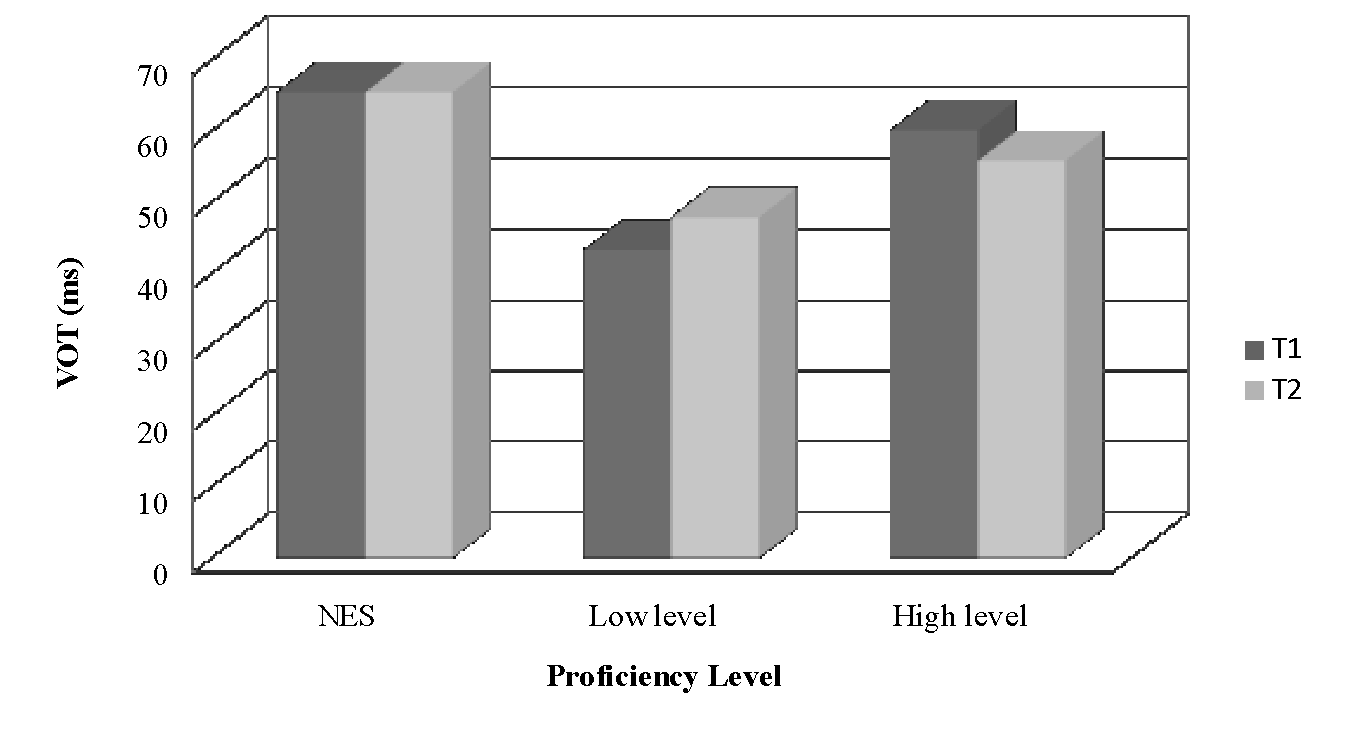
\includegraphics[width=\textwidth]{figures/monje-img4.png}

  \begin{tikzpicture}
    \begin{axis}[
	xlabel={Proficiency level},  
	ylabel={\isi{VOT} (ms)}, 
	axis lines*=left, 
        width  = .7\textwidth,
	height = .3\textheight,
    	nodes near coords, 
	xtick=data,
	x tick label style={},  
	ymin=0,
	ybar,
 	bar width=10mm,
	enlarge x limits=0.25,
	symbolic x coords={NES, Low level, High level},
	legend style={at={(1,0.4)},anchor=west}
	]
	\addplot+[ybar,lsLightBlue!80!black,fill=lsLightBlue] plot coordinates {
	    (NES, 65.47 ) (Low level,  43.27) (High level,60.11 )
	}; 
	\addplot+[ybar,lsMidBlue!80!black,fill=lsMidBlue] plot coordinates {
	    (NES,65.47 ) (Low level, 47.87) (High level,55.83)
	}; 
	\legend{T1, T2}
    \end{axis} 
  \end{tikzpicture} 
  
  
\caption{\label{fig:monje:4} Mean VOT measurements (ms) as a function of proficiency level}
\end{figure}
 






Interestingly, it can be observed in \tabref{tab:monje:5}  that the high-level group obtained numerically higher and more native-like \isi{VOT} values than the low-level group at the outset of the study, that is, after the SA period. This result might point towards a tendency of language experience to have a potential impact on \isi{L2} \isi{phonological} category learning, as predicted by the SLM. Along these lines, the more advanced group experienced stronger effects of category learning than the least experienced group, as a result of the SA period. 



  Looking more closely at the performance of both groups over time, the lower level group shows the largest improvement (43.27\% to 47.87\%). In fact, the higher \isi{proficiency} group experiences a slight numerical decrease in \isi{VOT} (60.11\% to 55.83\%). These results point to a tendency for improvement for the lower level group, while the tendency points in the opposite direction for the high-level group. These results, even though drawn from a small sample, may suggest that the high-level group had reached their ceiling \isi{VOT} values during the SA period, whereas the lower level group still had room for improvement. A potential reason for this is that the likely \isi{L2} categories formed by the high-level group for the target segments are more robust than those of the low-level group. Therefore, the \isi{FI} period following the SA might have been more effective in enhancement of \isi{L2} \isi{VOT} production for the low-level group than for their more advanced counterpart. This numerical tendency found in our data is in line with \citegen{Collentine2009} notion of a \textit{threshold} \textit{level.}



  Thus, it can be said that \isi{proficiency} level seems to play a significant role in the \isi{VOT} production of \ili{English} \isi{plosive} consonants in initial stressed position by \ili{Catalan}/\ili{Spanish} \isi{EFL} learners, at least as far as the effects of an \isi{FI} period following a SA period are concerned. However, given the small sample size and the lack of inferential statistical analysis, this study should be seen as mainly exploratory.



\subsection{Sub-research question 1.2.}



In order to explore whether the \isi{VOT} values obtained significantly differ as a \isi{function of task type}, a Wilcoxon-test was performed on the non-native data. As shown in \tabref{tab:monje:6} and \figref{fig:monje:5}, for both the non-native and the native groups, the \isi{VOT} durations produced when reading the text were significantly shorter than those obtained during the carrier sentence task at both times (\textit{z} = 2.830, \textit{N} = 13, \textit{p} = .0025, one-tailed) as well as at T1 (\textit{z} = 2.621, \textit{N} = 13, \textit{p} = .0045, one-tailed) and at T2 (\textit{z} = 2.900, \textit{N} = 13, \textit{p} = .002, one-tailed). 

\begin{table}
\caption{\label{tab:monje:6} Mean VOT measurements (ms) as a function of task (text vs. words)}
\begin{tabularx}{\textwidth}{l rrrr rrSr} 
\lsptoprule
&& \multicolumn{4}{c}{\textbf{Non-native speakers}} &&\multicolumn{2}{c}{\multirow{2}{2.8cm}{\centering\textbf{Native\newline \ili{English} speakers}}}\\
& \multicolumn{2}{c}{\textbf{T1}} & \multicolumn{2}{c}{\textbf{T2}} & \multicolumn{2}{c}{\textbf{T1+T2}} & \\
&\textbf{ms} &  \textbf{(sd)} & \textbf{ms} &  \textbf{(sd)} & \textbf{ms} & \textbf{(sd)}& \textbf{ms} & \textbf{(sd)}\\
\midrule 
{ {Words}} & 54.93 & (23.55)  & 55.07 &(20.13) & 55.00& (20.91) & 67.96& (29.87)\\
{ {Text}}  & 40.99 & (14.55)  & 42.40 &(13.98) & 41.69& (13.28) & 59.06& (13.54)\\
\lspbottomrule
\end{tabularx}
\end{table}                                 

  
\begin{figure}
% 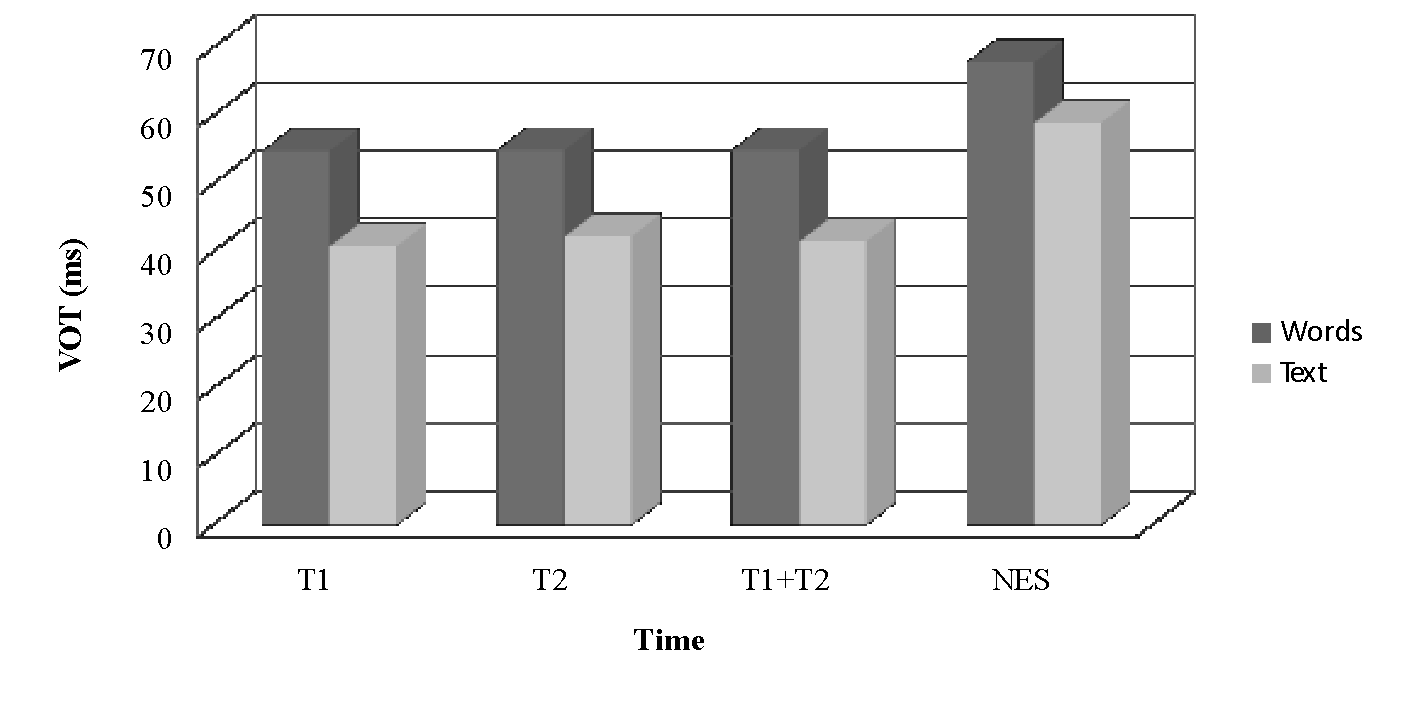
\includegraphics[width=\textwidth]{figures/monje-img5.png}
  \begin{tikzpicture}
    \begin{axis}[
	xlabel={Time},  
	ylabel={\isi{VOT} (ms)}, 
	axis lines*=left, 
        width  = .8\textwidth,
	height = .3\textheight,
    	nodes near coords, 
	xtick=data,
	x tick label style={},  
	ymin=0,
	ybar,
 	bar width=8mm,
	enlarge x limits=0.25,
	symbolic x coords={T1, T2, T1+T2, NES},
	legend style={at={(1,0.4)},anchor=west}
	]
	\addplot+[ybar,lsLightBlue!80!black,fill=lsLightBlue] plot coordinates {
	   (T1,54.93) (T2,55.07) (T1+T2,55.00) (NES,67.96) 
	}; 
	\addplot+[ybar,lsMidBlue!80!black,fill=lsMidBlue] plot coordinates {
	   (T1,40.99) (T2,42.40) (T1+T2,41.69) (NES,59.06) 
	}; 
	\legend{Words, Text}
    \end{axis} 
  \end{tikzpicture} 
  
\caption{\label{fig:monje:5} Mean VOT measurements (ms) as a function of task (text vs. words)}
\end{figure}
 






The results presented here suggest that speaking style significantly affects the \isi{VOT} production of \ili{Catalan}/\ili{Spanish} learners of \ili{English}, answering \isi{sub-research question} 1.2. Despite the lack of statistical differences between the native and non-native groups, the numerical values obtained from the natives suggest that speaking style affected both our groups of participants similarly. Our hypothesis is thus confirmed. Our data support \citegen{Labov1972} original idea that speaking style does have an effect on \isi{pronunciation} and more specifically on \isi{VOT} production, as also found by \citet{Mora2008} and \citet{Bach2012}, confirming that in continuous speech, \isi{VOT} values tend to decrease, whereas they tend to increase when produced in (quasi-)isolation. 



\subsection{Sub-research question 1.3.}



With the purpose of determining whether there are differences in the \isi{VOT} values as a function of the height of the \isi{vowel}, another Wilcoxon-test was conducted. As observed in \tabref{tab:monje:7} and \figref{fig:monje:6}, VOTs produced preceding a high \isi{vowel} were longer than those followed by a low \isi{vowel} both for the native and the non-native speakers. The test on the non-\isi{native speaker} data revealed that this difference did reach statistical significance between the \isi{VOT} values of high and low vowels (\textit{z} = 3.180, \textit{N} = 13, \textit{p}= .0005, one-tailed).


\begin{table}
\caption{\label{tab:monje:7} Mean VOT measurements (ms) as a function of vowel height averaged across time (T1+T2).}


\begin{tabularx}{\textwidth}{X rrSr}
\lsptoprule
& \multicolumn{2}{c}{\textbf{Non-native speakers}} & \multicolumn{2}{c}{\textbf{Native \ili{English} speakers}}\\
&\textbf{ms} &  \textbf{(sd)} & \textbf{ms} &  \textbf{(sd)}\\
\midrule 
 {High vowel} & 56.52 &(18.04) & 71.51& (25.75)\\
 {Low vowel} & 46.25 &(18.96) & 59.72 &(24.18)\\
\lspbottomrule
\end{tabularx}
\end{table}

  
\begin{figure}
% 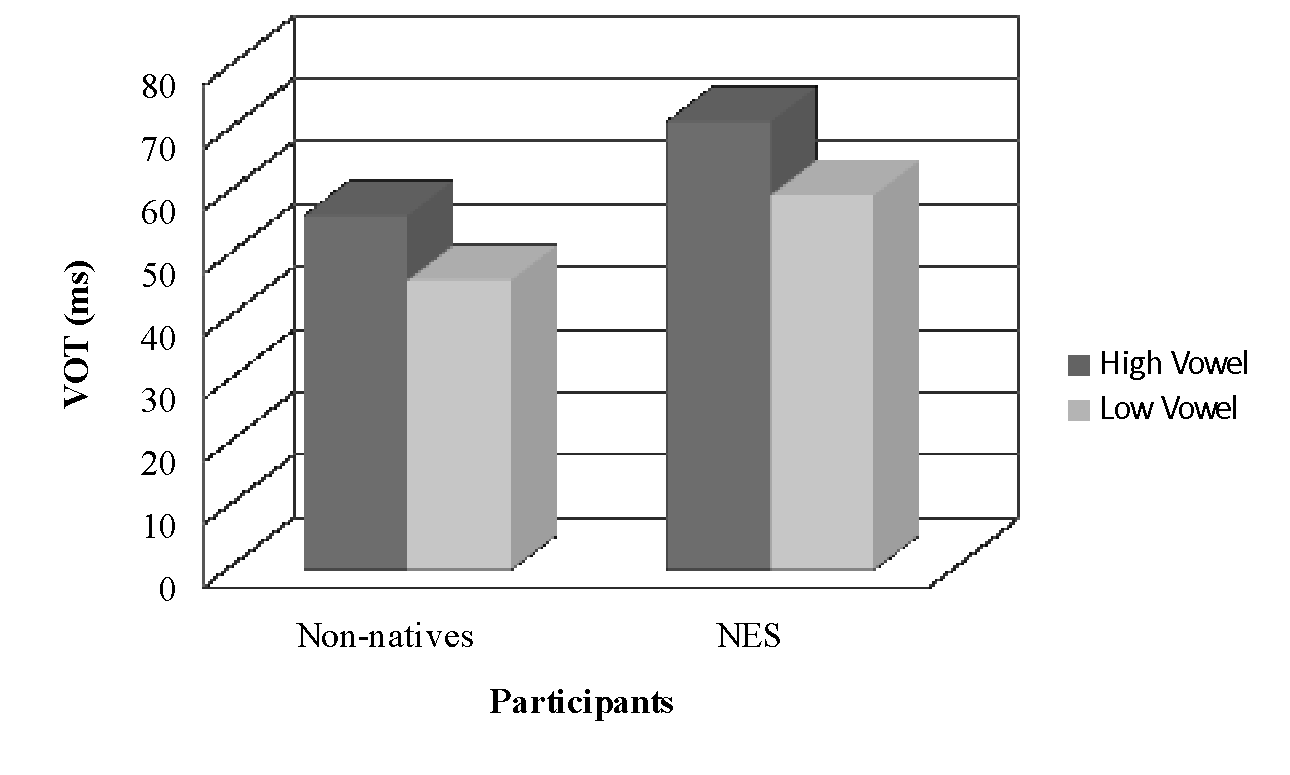
\includegraphics[width=\textwidth]{figures/monje-img6.png}
  \begin{tikzpicture}
    \begin{axis}[
	xlabel={Participants},  
	ylabel={\isi{VOT} (ms)}, 
	axis lines*=left, 
        width  = .5\textwidth,
	height = .3\textheight,
    	nodes near coords, 
	xtick=data,
	x tick label style={},  
	ymin=0,
	ybar,
 	bar width=8mm,
	enlarge x limits=0.5,
	symbolic x coords={Non-natives, NES},
	legend style={at={(1,0.4)},anchor=west}
	]
	\addplot+[ybar,lsLightBlue!80!black,fill=lsLightBlue] plot coordinates {
	   (Non-natives,56.52) (NES,71.51) 
	}; 
	\addplot+[ybar,lsMidBlue!80!black,fill=lsMidBlue] plot coordinates {
	   (Non-natives,46.25) (NES,59.72) 
	}; 
	\legend{High \isi{vowel}, Low vowel}
    \end{axis} 
  \end{tikzpicture} 
  
\caption{\label{fig:monje:6} Mean VOT measurements (ms) as a function of vowel height averaged across time (T1+T2).}
\end{figure}
 


These results suggest that \isi{vowel} height does have a significant effect on \isi{VOT} production of \ili{Catalan}/\ili{Spanish} learners of \ili{English}, answering \isi{sub-research question} 1.3. Interestingly, a similar pattern was observed for the native speakers. The hypothesis formulated regarding this sub-RQ is confirmed by the data and in line with \citet{FlegeEtAl1998} and \citegen{YavaşWildermuth2006} findings that \isi{vowel} height does influence \isi{VOT} production. 



\subsection{Sub-research question 1.4.}



To determine whether \isi{VOT} values differed as a function of place of articulation, three Wilcoxon-tests were run on the data obtained from non-native speakers. As shown by \tabref{tab:monje:8} and \figref{fig:monje:7}, /k/ displayed the longest \isi{VOT} values, with /t/ in the second place and /p/ having triggered the shortest durations for the non-native group. However, natives produced slightly longer VOTs for /t/ than for /k/. In turn, \isi{VOT} values for /p/ were the shortest for this group.


\begin{table}
\caption{\label{tab:monje:8} Mean VOT measurements (ms) as a function of place of articulation averaged across time (T1+T2).}


\begin{tabularx}{\textwidth}{Q rrrrrr} 
\lsptoprule
&\multicolumn{2}{c}{K} & \multicolumn{2}{c}{T} & \multicolumn{2}{c}{P} \\
&\textbf{ms} &  \textbf{(sd)} & \textbf{ms} &  \textbf{(sd)} & \textbf{ms} &  \textbf{(sd)}\\
\midrule 
 {Non-native speakers}           & 61.62& (20,17) & 57.50 &(22.09) & 35.78 &(15.26)\\
 {Native \ili{English} speakers} & 70.44& (24.68) & 72.79 &(22.81) & 54.01 &(27.28)\\
\lspbottomrule
\end{tabularx} 
\end{table}




  
\begin{figure}
% 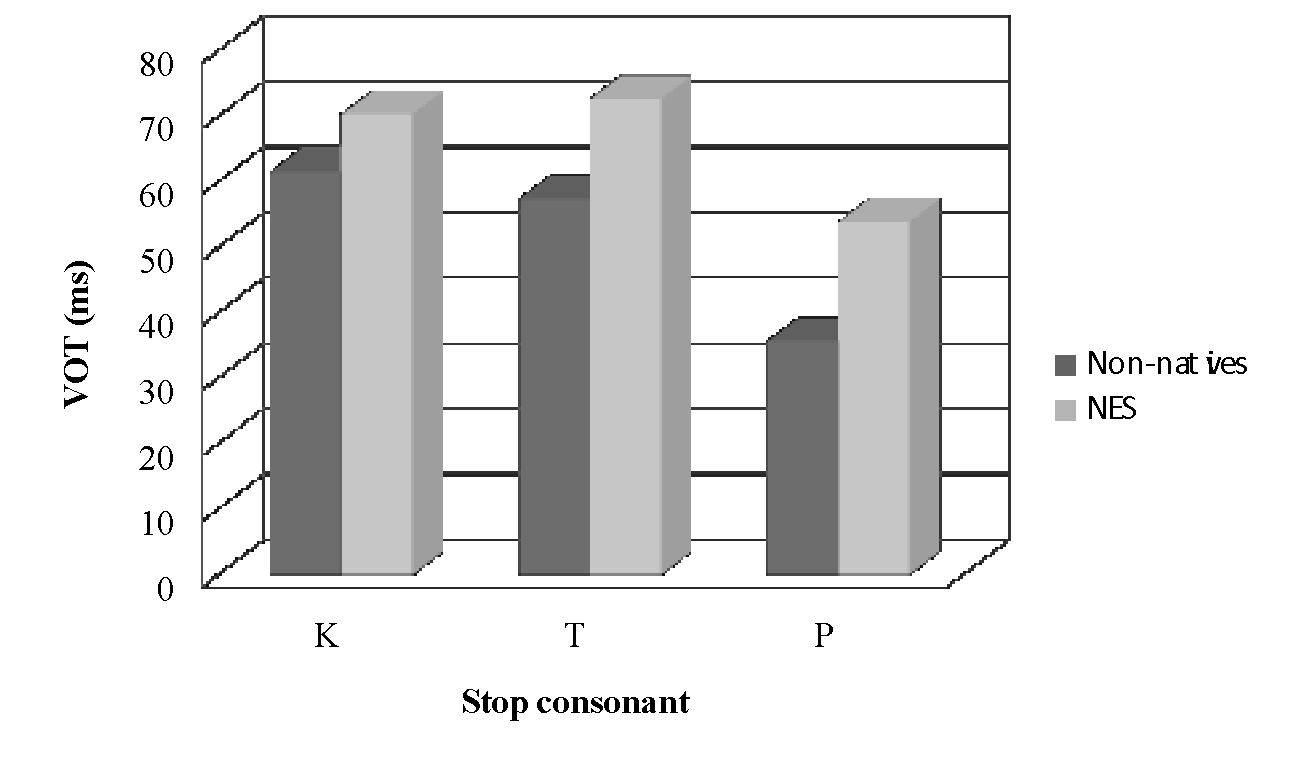
\includegraphics[width=\textwidth]{figures/monje-img7.png}
  \begin{tikzpicture}
    \begin{axis}[
	xlabel={Stop consonant},  
	ylabel={\isi{VOT} (ms)}, 
	axis lines*=left, 
        width  = .8\textwidth,
	height = .3\textheight,
    	nodes near coords, 
	xtick=data,
	x tick label style={},  
	ymin=0,
	ybar,
 	bar width=8mm,
	enlarge x limits=0.5,
	symbolic x coords={K,T,P},
	legend style={at={(1,0.4)},anchor=west}
	]
	\addplot+[ybar,lsLightBlue!80!black,fill=lsLightBlue] plot coordinates {
	   (K,61.62) (T,57.50) (P,35.78)
	}; 
	\addplot+[ybar,lsMidBlue!80!black,fill=lsMidBlue] plot coordinates {
	   (K,70.44) (T,72.79) (P,54.01)
	}; 
	\legend{Non-natives, NES}
    \end{axis} 
  \end{tikzpicture} 
\caption{\label{fig:monje:7}  Mean VOT measurements (ms) as a function of place of articulation averaged across time (T1+T2).}
\end{figure}
 






The test revealed that \isi{VOT} values obtained for /p/ were significantly different from those obtained for /k/ (\textit{z} = 3.180, \textit{N} = 13, \textit{p} = .0005, one-tailed) and for /t/ (\textit{z} = 3.180, \textit{N} = 13, \textit{p} = .0005, one-tailed), respectively. However, \isi{VOT} values obtained for /k/ and /t/ were not significantly different from one another (\textit{z} = 1.223, \textit{N} = 13, \textit{p} = .1105, one-tailed).  



  The relative similarity of \isi{VOT} values for /k/ and /t/ might be explained by the fact that they are quite similar in native speakers as well. Moreover, according to \citet{AlvesZimmer2015}, aspiration is a cue that learners pay attention to, which might explain why the \isi{VOT} values for /k/ and /t/ did not to reach statistical significance in the present study. Specifically, it is more salient in some places of articulation than in others. This seems to indicate that our participants are in the process of creating \isi{L2} categories for the target segments, as their performance shows certain similarities with that of the baseline group. Although their \isi{VOT} durations never reach those produced by the natives, as predicted by the SLM, the initial hypothesis that place of articulation affects \isi{VOT} (\citealt{YavaşWildermuth2006}) is confirmed.



\section{Summary and conclusions}


The present study aimed at making a contribution to the SALA project by providing a study not undertaken before. Moreover, it sought to reduce the present research gap in the field of \isi{L2} \isi{phonology} \isi{acquisition} during SA in combination with a subsequent \isi{FI} period. It sought to examine and measure the effects of a 2-month \isi{FI} period, with no specific training in the learners’ \isi{L2} \isi{phonological} abilities, preceded by a 3-month long SA term, on the \isi{VOT} production by \ili{Catalan}/\ili{Spanish} \isi{EFL} learners.



  Results revealed that a 2-month \isi{FI} period preceded by a 3-month long SA term undergone by our participants had no statistically significant effects on their \isi{VOT} production of \ili{English} \isi{voiceless} \isi{plosive} consonants, although a tendency towards improvement was observed. Such findings might be due to the limited statistical power of this exploratory study, but they may also lead one to reflect on the absence of \isi{explicit instruction} on \isi{L2} \isi{phonology} which characterises most \isi{FI}.  We are thus led to wonder whether an \isi{FI} with \isi{explicit instruction} on \isi{L2} \isi{phonology} would have a positive effect on \isi{L2} \isi{phonological} \isi{acquisition} in \isi{EFL} learners.



  Moreover, \isi{proficiency} level might play a role on \isi{VOT} production, given that the high level group displayed higher values than the low level one, although this was not statistically confirmed. In addition, ceiling effects were found in the advanced group, whereas the lower level group seemed to have more room for improvement. These findings must tentatively be taken as tendencies. On the other hand, speaking style, \isi{vowel} height, and place of articulation do significantly affect \isi{VOT} production of \isi{voiceless} plosives by \ili{Catalan}/\ili{Spanish} learners. The native group displayed a similar numerical pattern, which indicates that these three independent factors affect both groups in a similar way. However, natives always produce higher \isi{VOT} values for \ili{English} \isi{voiceless} stops, confirming that \isi{EFL} learners tend to produce intermediate \isi{VOT} values between their L1 and their \isi{L2} for the same consonants. As for speaking style, words in (quasi-)isolation (carrier sentence task) displayed significantly higher values than those produced in continuous speech (read aloud task). We might interpret these results by stating that the more attention is paid when uttering words, the more likely the sounds produced are to be clearly articulated. As for \isi{vowel} height, \isi{VOT} values produced before a high \isi{vowel} were significantly longer than those produced preceding a low \isi{vowel}. Finally, concerning place of articulation, VOTs for /k/ displayed the highest values, with /t/ in the second place and values for /p/ being the shortest. It must be stressed that only the /k/ vs. /t/ comparison failed to reach statistical significance. The results concerning place of articulation can be understood through the SLM. Our participants seem to be in the process of creating \isi{L2} categories for \isi{voiceless} stops, as they performed similarly to the native group regarding the lack of difference between /k/ and /t/. This suggests that aspiration is more salient in some places of articulation than in others \cite{AlvesZimmer2015}.



\section{Limitations and directions for prospective research}


In this final section, we identify some of the limitations of the current study and highlight directions for future research. When work on this study started, it was no longer possible to test participants prior to their experience abroad, and thus \isi{VOT} measurements before SA could not be obtained. The reason is that informants were already abroad by data collection T1. Hence, all collected data were gathered only after the SA period, so the obtained VOTs cannot be contrasted against those prior to SA, which would presumably have provided valuable information as for the learners’ \isi{VOT} departure values.



One other issue is the measurement of \isi{proficiency} level. Testing should have been conducted at both data collection times, and not only at T2. Time constraints prevented this from happening. 



In addition, the number of participants was low, both for the non-native and the native groups. This prevented us from drawing general conclusions and accentuates the fact that conclusions related to our population must be taken with caution. Finally, the native speakers who served as a baseline group are not monolingual, so their \isi{VOT} values might have been influenced by other languages. However, all of them are late bilinguals.



  Despite the lack of statistical reliability for some of the tendencies we found, they leave a door open to prospective research, namely with a larger population so that more robust claims can be made. A further study should measure the effects of a post-stay-abroad \isi{FI} period including either \isi{explicit instruction} on \isi{L2} \isi{phonology} or \isi{L2} \isi{phonetic} training and focusing either on the \isi{VOT} of \ili{English} stops or on other relevant acoustic cues.


 
\sloppy
\printbibliography[heading=subbibliography,notkeyword=this] 
\end{document}